\chapter{Starting and ending university enrolment} \label{chap:1}


As higher education enrolments have increased in recent decades, dropping out of university has become a common experience for Australians. In 2015, the ABS estimated that 800,000 Australian had started but not finished a degree at some time. That number is growing by more than 50,000 a year.

Australian public policy makes it cheap and easy to give university a try, and for many young people that is now the default option after leaving school. Some of them only find out after they commence their studies whether university is for them. For universities, it can be hard to tell the applicants who are committed to getting a degree from the applicants who are just exploring their options.

This chapter explains the implications of that uncertainty faced by both students and universities. It shows that the selection of students by universities, and the first semester or two of enrolment, are not two entirely distinct phases. Instead, they overlap.

\section{Starting university and mutual selection }\label{sec:1.1}

                % Figure 1
                \begin{figure}
                    \caption{School-leaver application rates decline as ATAR declines\label{fig:1}}%
                    \units{Proportion of school students applying for university through a tertiary admission centre, per cent, by ATAR, 2014}
                    \includegraphics[page=3]{atlas/selection_chartdeck.pdf} 
                    \noteswithsource{Excluding direct applications to universities and Queensland students, since Queensland primarily uses Overall Position rather than ATAR\@. The population is based on Year 7 students in 2008. Only applicants who studied Year 12 in 2013 who have an ATAR\@. ATAR is a rank of all people in the age cohort. Actual ATARs awarded are skewed to the higher end, because students who would have received the lower ATARs left school before Year 12 or did not receive an ATAR\@.}
                    {\textcite{ABSc}; \textcite{DepartmentofEducationandTraininga}}
                \end{figure}



People's decision-making about university often starts during childhood, when they begin forming views about their post-school education and careers.\footcites[][]{Gore2017a}[][]{Gore2017b}[][51]{RoyMorganResearch2009} 
At least since the 1990s, most upper-years school students in Australia have indicated an interest in going to university.\footcites[][15]{James2002}[][15--16]{MissionAustralia2016}[][48--50]{RoyMorganResearch2009}[][7--9]{ANOP/DEET1994} 
By the end of Year 12, this interest is moderated by academic results. As \Cref{fig:1} shows, a school leaver's propensity to apply for university declines with their ATAR, reflecting their preference for academic work, how likely they are to receive an offer, and their chances of success at university.

Despite ATAR's moderating effect on interest in higher education, most Year 12 students apply for university. But not all Year 12 applicants are strongly committed to university in general or a particular course. Surveys clearly show student indecision about their course and university choice. South Australian research into Year 12 student decision-making found that one-in-five were uncertain about their university preferences, but were going to apply anyway, and only 60 per cent were certain or very certain about their first preference.\footcite[][8]{Parks2017}

Similarly, a 2015 survey of first-year students at two universities found that less than two-thirds believed they had a good or very good understanding of which course would be best for them.\footcite[][58]{Harvey2016} 
A 2014 survey of first-year university students found 4 per cent were unclear about why they were at university, and 20 per cent agreed with the proposition that they were `marking time'.\footcite[][31]{Baik2015} 
A small percentage of students who drop out say that they never really intended to complete.\footnote{See \Vref{fig:26}.}
The decisions of young people are often driven by strong parental and social expectations around university attendance, not clear or definite goals.\footnote{Of first year students in 2004, 41 per cent cited parental expectations as a factor, and 65 per cent cited school pressure as a factor in their decision to go to university: \textcite[][22]{Baik2015}.} For them, university is now a default option.

Ultimately many students drop out, although saying exactly what proportion do so is not straightforward. Calculating a drop-out rate requires identifying a start and a finish date for each student. A student's first day of enrolment is an obvious starting point, but it is not used to calculate Australian attrition or completion rates. Students are only counted if they remain enrolled at a `census date', which is at least 20 per cent of the way through the semester.\footcite[][section~6.30]{DIICCSRTE2013} 
Students often enrol well before the teaching period begins, so the census date could be two months or longer after enrolment.

While it could seem that this late start date under-states attrition rates, it recognises that the time immediately after enrolment is not entirely distinct from the prior period, when prospective students look for courses and universities decide whether to admit them. In practice, the selection and enrolment phases overlap in a long process of mutual selection, during which prospective students and universities decide whether the student will proceed in a course.


Australia's student selection system does little to discourage speculative applications from people without clear aims. For a modest fee, usually well below \$100, prospective students can apply simultaneously for multiple courses through tertiary admissions centres in each state. Applicants receive offers, if any, in order of their stated preferences. The process lets applicants keep their options open at low cost. It gives them more time to decide, and more time perhaps to find something they would like more, such as a job.

For the potential students who do apply, universities must decide whether to offer them a place. The applicant's prospect of success is almost always an explicit selection principle.\footnote{Based on desktop research in January 2018.} What prospect of success each university regards as acceptable is not clear, but the criteria for assessing it are primarily academic (discussed further in \Cref{sec:4.2}). Many universities set minimum ATARs, varying from 50 to 80, depending on the university. When the applicant has been to university before, previous academic results are often used. Special admissions tests, auditions, professional experience and vocational education are also used as admission criteria.

Some applicants receive no offers. \Vref{fig:2} uses applicants for the 2014 academic year as a guide to what proportion of the original applicants leave at each stage in the mutual selection process. Seventeen per cent of the original pool were screened out by the offers process. The share varies slightly depending on applicant type. Applicants who finished Year 12 in 2013 were slightly more likely to receive an offer than older applicants.

Inevitably, applications data lacks important information relevant to a university decision about applicants' prospects of success. Although applicants with unrealistic plans often have warning signs (\Chapref{chap:3}), these are not conclusive. The committed applicant who is determined to succeed, and the uncommitted applicant who is just keeping options open, can look very similar. Universities cannot fully identify which category an applicant is in before making offers.

The offers process itself identifies some uncertain applicants. Overall, 8 per cent of the original applicant pool selected itself out by not accepting their offer. Disappointment may be a factor for applicants who did not receive an offer for their first-preference course.\footnote{Applicants were 8 percentage points more likely to accept if offered their first- rather than their second-preference course, and 15 percentage points more likely to accept if offered their first- rather than their third-preference course: \textcite[][]{DepartmentofEducationandTraining2017n}.} But first-preference offers were also rejected, indicating some applicants had second thoughts, and some were never very serious about university. People who had just completed school were more likely to proceed than older applicants, perhaps because they are under more social pressure to study and have fewer other demands on their time.

Uncertain applicants can extend their decision time into first semester. Accepting and enrolling does not of itself trigger financial costs. Students are not charged unless they are still enrolled on the census date (discussed in more detail in \Chapref{chap:6}). For people who are unsure about university, this free try-before-you-buy period gives them added information supplied by their initial university experiences.\footnote{Universities vary in their enrolment practices. Some combine accepting offers and enrolment, while at others accepting an offer and enrolling are separate processes. At these universities, some applicants may never have enrolled despite accepting their offer.} Overall, another 7 per cent of the original applicant pool selected itself out by the first semester 2014 census date. Again, younger and older applicants behaved differently, with those who had just completed school more likely to persist at university.

About one-third of the original applicant pool departed by the first semester census date. Exit decisions were distributed fairly between universities and applicants; universities made no offer to 17 per cent of applicants, and 16 per cent of applicants did not accept their offer or left before the census date.\footnote{The proportion of applicants who did not accept their offer (8.3 per cent) or left before the census date (7.4 per cent) was 15.7 per cent.}

                
                % Figure 2
                \begin{figure*}
                    \caption{A mutual selection process decides who will continue with their course\label{fig:2}}%
                    \units{Applicants for the 2014 academic year}
                    \includegraphics[page=2, width=2.15\columnwidth]{atlas/transition_fullpage.pdf} 
                    \noteswithsource{2014 domestic bachelor applicant cohort only. Those who completed high school in 2013 are considered school leavers. Applications to tertiary admission centres and direct applications are considered. Only those who accept or defer an offer are considered in the enrolment stages. Second year is equivalent to the third and fourth semesters after commencing studies. Applications to UAC (NSW) and UTAS (Tasmania) have a high proportion of `offer response unknown' observations and been omitted from the analysis. The analysis only includes applicants, enrolments and completions in bachelor courses. See \Chapref{chap:a} for detailed methodology.}
                    {\textcite{DepartmentofEducationandTraininga}}
                \end{figure*}


Having reached the census date, students become liable to pay student contributions. For some, letting the census date pass without action is a mistake; they have disengaged but not disenrolled, and needlessly pay for their subjects. How to minimise this is discussed in \Chaprefand{chap:6}{chap:8}. But others continue experimenting with university, deciding whether it is for them. Surveys asking departed students why they left show substantial proportions giving reasons such as the course being different from what they wanted, not gaining or keeping their interest, and being too hard.\footnote{See the survey results reported in \Chapref{chap:b}.} Of the original applicant pool, another 8 per cent left after first semester. Again, school leavers are more likely to stay than older students. This pattern is repeated at the end of first year. In the second academic year, just over half of the original applicant pool remain.

During the academic year, universities again play a critical role in the mutual selection process. Students use initial academic results as feedback in their decision-making. In 2014, 8 per cent of commencing bachelor degree students failed all their first semester subjects, and another 18 per cent failed some subjects.\footnote{Including those taking only one subject: \textcite[][]{DepartmentofEducationandTraininga}.} 
Bad results can trigger voluntary departures, perhaps among students who were originally clear about their direction, as well as those who were uncertain all along.\footnote{The annual Student Experience Survey is conducted in August, when many of the original pool of people who accepted their offer have already left. However, unsurprisingly it shows that students reporting low average marks are much more likely to be considering early departure than those getting high average marks: \textcite[][11]{SocialResearchCentre/DepartmentofEducationandTraining2017}.} 
Universities prompt disengaged students to consider withdrawing from their studies. But not all the later departures reported in \Cref{fig:2} are voluntary. Universities can exclude students who persistently fail subjects; this process usually begins at the end of first year. \Chaprefand{chap:6}{chap:8} consider these parts of the selection process in more detail.

Which start date is used has substantial implications for calculating drop-out rates. If the start date was accepting an offer for a bachelor degree place in 2014, 24 per cent of students were not enrolled at any public university in second year. If the start date was the first semester census date, the date used in official statistics, 15 per cent were not enrolled in second year. If the start date was the second semester census date, after many students enrolling on a speculative or experimental basis have either gone or committed to continuing, only 9 per cent were not enrolled in second year.

Each measure has potential uses, but needs to be evaluated in the context of policy incentives and goals. If prospective students were charged a substantial fee for applying, fewer would do so; if student contributions were charged on accepting or enrolling, fewer applicants would accept their offer. The system encourages potential students to keep their options open and give university a try. Whether this process could be more efficient, while preserving an open system, is discussed in later chapters.


\section{ Ending university}\label{sec:1.2}

Just as there are several potential university start dates, there are several potential end dates. Students can change courses or take time off but still end up completing a degree, so early end dates can misclassify individuals. Some students classified as departed in \Cref{fig:2} will return in a later year, while others classified as retained will subsequently leave without a degree.

In the shortest-run currently-published statistics, the Department of Education and Training counts as attrition a commencing student who reached their first census date but is not enrolled the next calendar year and has not completed their course. The higher education regulator, the Tertiary Education Quality and Standards Agency (TEQSA), monitors each university's year-to-year commencing student attrition statistics.\footcite[][]{TEQSA2016e} 
While attrition statistics do not measure final completions, they are a useful trend indicator that can quickly reveal potential problems. An institution's commencing student attrition rate is highly correlated with its long-term completion rate.\footnote{In separate analysis of commencing students between 2006 and 2008, the correlation between first-year attrition and completion within nine years is about 90 per cent.}

Students can still complete a degree long after starting.\footnote{Universities typically have maximum completion times between seven and ten years for a bachelor degree course. However, students can move to another university.} 
In addition to attrition rates, the Department produces completion statistics over four, six and nine-year periods.\footcite{DepartmentofEducationandTraining2017} 
In practice, few students complete after eight years.\footnote{An eight-year timeframe lets us look at more student cohorts than longer timeframes. Data was only available for the years 2005 to 2015, limiting the scope for 9- or 10-year cohorts. About an additional 2 per cent of students are expected to complete in years 9 and 10. Our data does not extend further, but some students may eventually return after longer periods.} 
This report's main statistical analysis uses an eight-year completion timeframe, covering domestic students who commenced a bachelor degree in a public university between 2006 and 2008. On this measure, 70 per cent of students who commenced in 2008 completed within eight years (\Cref{fig:3}). Another 7 per cent had been enrolled in at least one of the last two years, while just under a quarter had neither completed a bachelor degree nor been enrolled in either of the last two years.

                % Figure 3
                \begin{figure}
                    \caption{Three in every ten students do not complete a degree within eight years\label{fig:3}}%
                    \units{Proportion of bachelor degree students who commenced in 2008}
                    \includegraphics[page=5]{atlas/selection_chartdeck.pdf} 
                    \noteswithsource{Commencing domestic students with a Commonwealth Higher Education Student Number (CHESSN) who first enrolled in 2008. CHESSN is used to track students over time. `Completed' includes any bachelor degree completion, including students completing a degree in a different field or at a different institution from the one they started. `Still enrolled' includes students who were enrolled in the 7\textsuperscript{th} or 8\textsuperscript{th} year after they commenced, or both. `Left' is classified as students who have not completed and were not enrolled in the 7\textsuperscript{th} or 8\textsuperscript{th} year after they enrolled. Bachelor graduate entry students, permanent humanitarian visa-holders, students studying entirely offshore, and students who completed in the same year they commenced are excluded (less than 3 per cent).}
                    {Grattan analysis of \textcite{DepartmentofEducationandTraininga}}
                \end{figure}

Another measure again is to take the degree length and then add some time. Anyone who finishes within this period is counted as a completion; everyone else is a non-completion. The OECD uses this method. On this measure, Australia's non-completion rate is about average in the OECD.\footnote{Based on the theoretical length of the degree plus three years for full-time students: \textcite[][166--170]{OECD2016}.}

\section{Trends in completion rates}\label{sec:1.3}


                \doublecolumnfigure {
                % Figure 4
                
                    \caption{Completion rates are deteriorating slightly\label{fig:4}}%
                    \units{Proportion of students completing a bachelor degree by year of commencement, per cent}
                    \includegraphics[page=6]{atlas/selection_chartdeck.pdf} 
                    %\includegraphics[page=4]{atlas/selection_deck_halfpage.pdf} 
                    \noteswithsource{Commencing domestic students with a CHESSN\@. Based on the first enrolment between 2006 and 2013 of each student. See \Cref{fig:3}.}
                    {Grattan analysis of \textcite{DepartmentofEducationandTraininga}}
                

                }{
                % Figure 5
                
                    \caption{Early student departures have trended up\label{fig:5}}%
                    \units{Proportion of students who did not return in second year to a bachelor degree, per cent}
                    \includegraphics[page=7]{atlas/selection_chartdeck.pdf} 
                    \noteswithsource{Students not retained in a bachelor degree at any university. The Department of Education and Training also publishes attrition time series: one showing the proportion of commencing students leaving each university, and another showing the proportion of students leaving the higher education system, \textcite[][appendix~4]{DepartmentofEducationandTraining2017a}. Due to transfers between universities, attrition from the system is lower than attrition from individual universities. The Department's system-level attrition number is lower than the numbers in this chart because it counts students who have downshifted to a diploma or associate degree and completions in those courses as enrolments. These are not counted in this chart.}
                    {Grattan analysis of \textcite{DepartmentofEducationandTraininga}}
                
                }


While Australia's completion rates are not unusual compared to other countries, they are decreasing slightly using the census date commencement method. \Vref{fig:4} suggests that compared to students commencing in 2008, subsequent students are slightly more likely to drop out. Whether we check progress at four, five or six years after commencement, the 2008 cohort has the highest completion rate of recent cohorts. The four-year analysis suggests that the deteriorating trend will continue until at least the 2013 cohort. The four-year completion rate of students commencing in 2013 was 4 percentage points below the result for the 2008 cohort.

\Vref{fig:5}, which reports on attrition after first year, suggests that long-term completions may decline further. Students were more likely to leave after their first year in 2015 compared to 2008, although with only a small upward trend since 2013, and an overall rate only slightly higher than it was in 2006.

While the \emph{share} of students leaving university without a qualification is not growing drastically, the \emph{number} of such students is growing substantially -- because about 40 per cent more people go to university now than in 2008.\footnote{The growth in unique CHESSNs for commencing enrolments between 2008 and 2014 at public universities was 40 per cent, \textcite{DepartmentofEducationandTraininga}.} Given that the additional students tend to have lower ATARs than typical students in the past (see \Vref{fig:20}), it is surprising that the growth in student numbers has not reduced completion rates even further.

In 2018, about 240,000 commencing domestic students are expected to enrol at Australia's public universities.\footnote{There were about 240,000 enrolments with a unique CHESSN public universities in 2016. Growth in commencing domestic bachelor degree student numbers slowed to close to zero in 2015 and 2016. Applications and offers statistics suggest another year of stable numbers in 2017. As a result, zero growth is assumed between 2016 and 2018 throughout this report, \textcite{DepartmentofEducationandTraining2017b}.} 
Even using the best recent commencing year for completions, 2008, as a guide, 23 per cent, or nearly 55,000 of these students, are likely to drop out. Given subsequent trends, the actual proportion is likely to be higher still. They will add to the large pool of people who have started but not finished a degree. In 2015, the Australian Bureau of Statistics (ABS) estimated that nearly 800,000 people had an incomplete bachelor degree (other than one they were currently enrolled in).\footnote{Calculated from \textcite{ABS2016f}. There are differences between the methodology used in this report and the ABS methodology. See \textcite[][section~1.2]{Cherastidtham2018a}.}

\section{Policy interest in course non-completion}\label{sec:1.4}

The Federal Government is concerned about increasing non-completion rates. The Education Minister, Senator Simon Birmingham, has asked the Higher Education Standards Panel, a statutory advisory committee, to look into the factors driving attrition, and how higher education providers can support student success and course completion.\footcite[][5]{HigherEducationStandardsPanel2017} 
He is making university funding partly contingent on university performance, including on retaining students (there is more on performance funding in \Vref{sec:8.3}).\footcite{AustralianGovernment2017c} 
TEQSA, responsible for ensuring higher education providers meet legal minimum standards on admission and student progress, has also investigated attrition levels (there is more on TEQSA in \Chapref{chap:7}).\footnote{Attrition levels: \textcite[][]{TEQSA2017e}. Minimum standards: \textcite[][]{DepartmentforEducationandTraining2015}.}

Government interest in attrition and completion is not misplaced -- in some cases dropping out leads to costs that are unnecessarily high, and benefits that are unnecessarily low. But there is a careful balance to maintain. As the next chapter will show, students who drop out receive benefits as well as incur costs.

